% ========================================
% Document Class and Package Setup
% ========================================
\documentclass[%
 reprint, amsmath,amssymb, aps, prb, ]{revtex4-2}
\setcounter{secnumdepth}{4}
\usepackage{graphicx}
\usepackage{bm}
\usepackage{physics}
\usepackage[colorlinks=true,
            linkcolor=blue, filecolor=blue, urlcolor=blue, citecolor=blue]{hyperref}
\usepackage{caption}
\captionsetup[figure]{
    justification=raggedright, labelfont={bf}, name={Fig.}, labelsep=period }
\captionsetup[table]{
    labelfont={bf}, name={Table}, labelsep=period }
\numberwithin{equation}{section}
\tolerance=1000
\emergencystretch=1em
\hyphenpenalty=3000
\exhyphenpenalty=3000
\flushbottom
\usepackage[final]{microtype}
\usepackage{ragged2e}
\usepackage{booktabs}
\usepackage{enumitem}
% Theorem environment
\usepackage{amsthm}
\newtheorem{theorem}{Theorem}[section]
\usepackage{xcolor}
\definecolor{backcolour}{rgb}{0.96,0.97,0.98}
\definecolor{deepblue}{rgb}{0,0,0.5}
\definecolor{deepgreen}{rgb}{0,0.5,0.3}
\definecolor{deepgray}{rgb}{0.4,0.4,0.4}
\usepackage{tikz}
\usetikzlibrary{arrows.meta, calc, positioning, shapes.geometric}

% --- Custom Macros ---
\newcommand{\vZB}{v_{\text{ZB}}}
\newcommand{\aexp}{a_{e}^{\text{exp}}}
\newcommand{\gammaL}{\gamma_{L}}
\newcommand{\Lzero}{L_{0}}

% ========================================
% TikZ Figure: Structural Comparison Diagram
% ========================================
\newcommand{\figComparison}{%
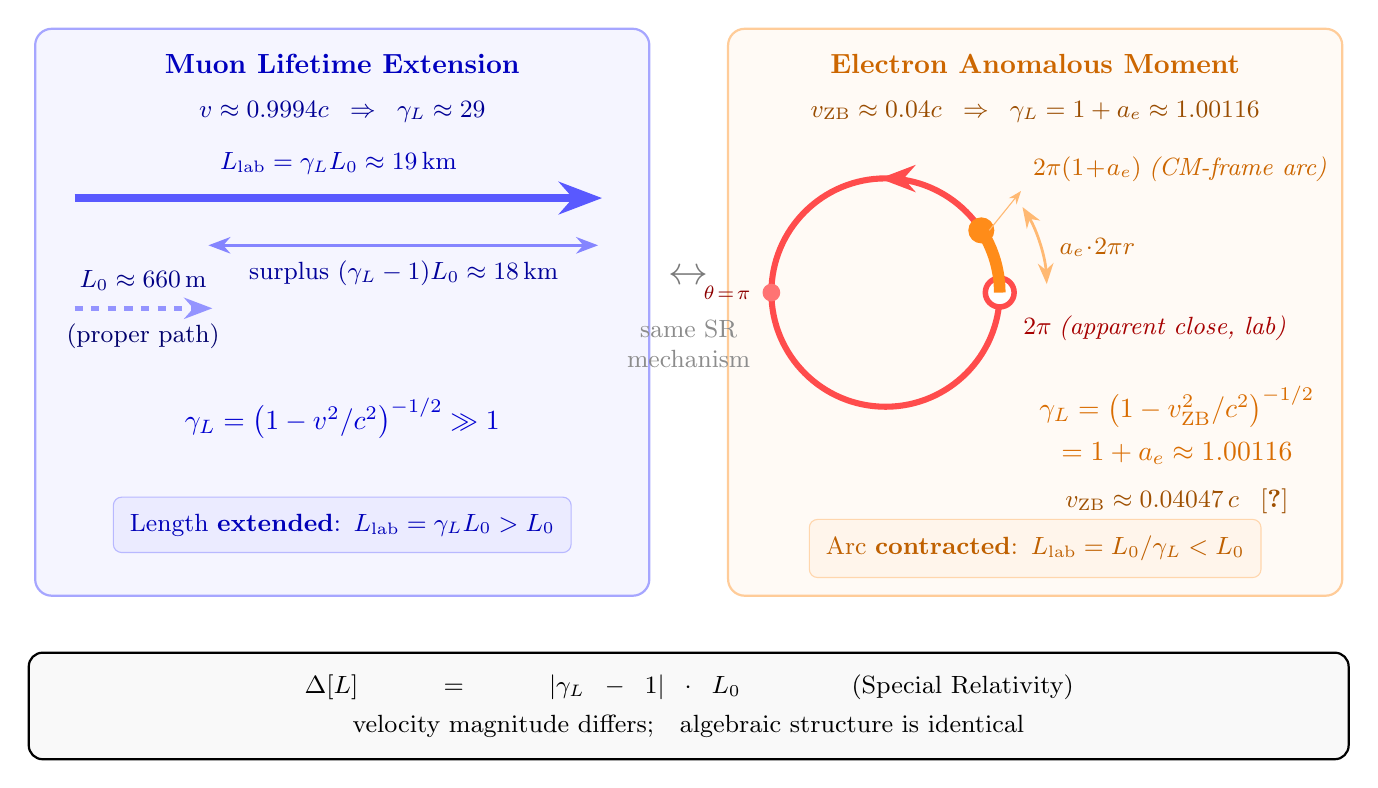
\begin{tikzpicture}[>=Stealth, font=\small]

%%====================================================
%% LEFT BOX — MUON LIFETIME
%% x in [-8.3, -0.5],  y in [-3.0, 4.2]
%%====================================================
\draw[thick, rounded corners=6pt, fill=blue!4, draw=blue!35]
  (-8.3, -3.0) rectangle (-0.5, 4.2);

%% Title + subtitle
\node[font=\normalsize\bfseries, blue!75!black] at (-4.4, 3.75)
  {Muon Lifetime Extension};
\node[font=\small, blue!58!black] at (-4.4, 3.15)
  {$v \approx 0.9994c$ \enspace $\Rightarrow$ \enspace $\gammaL \approx 29$};

%% L_lab: long solid arrow
\draw[->, blue!65, line width=2.8pt] (-7.8, 2.05) -- (-1.1, 2.05);
\node[above=5pt, font=\small, blue!72!black] at (-4.45, 2.05)
  {$L_{\text{lab}} = \gammaL L_0 \approx 19\,\text{km}$};

%% Surplus double-arrow (between end of L0 and end of L_lab)
\draw[<->, blue!48, line width=1.1pt] (-6.10, 1.45) -- (-1.15, 1.45);
\node[below=2pt, font=\small, blue!60!black] at (-3.62, 1.45)
  {surplus $(\gammaL-1)L_0 \approx 18\,\text{km}$};

%% L0: short dashed arrow (visually ~1/4 of L_lab)
\draw[->, blue!42, dashed, line width=1.6pt] (-7.8, 0.65) -- (-6.05, 0.65);
\node[above=3pt, font=\small, blue!52!black] at (-6.93, 0.65)
  {$L_0 \approx 660\,\text{m}$};
\node[below=2pt, font=\small, blue!42!black] at (-6.93, 0.65)
  {(proper path)};

%% gamma_L formula
\node[font=\normalsize, blue!82!black] at (-4.4, -0.75)
  {$\gammaL = \bigl(1 - v^2/c^2\bigr)^{-1/2} \gg 1$};

%% Key result
\node[draw=blue!28, rounded corners=3pt, fill=blue!8,
  font=\small, text=blue!72!black, inner sep=6pt] at (-4.4, -2.10)
  {Length \textbf{extended}:\enspace $L_{\text{lab}} = \gammaL L_0 > L_0$};

%%====================================================
%% RIGHT BOX — ELECTRON a_e
%% x in [0.5, 8.3],  y in [-3.0, 4.2]
%%====================================================
\draw[thick, rounded corners=6pt, fill=orange!4, draw=orange!40]
  (0.5, -3.0) rectangle (8.3, 4.2);

%% Title + subtitle
\node[font=\normalsize\bfseries, orange!80!black] at (4.4, 3.75)
  {Electron Anomalous Moment};
\node[font=\small, orange!60!black] at (4.4, 3.15)
  {$\vZB \approx 0.04c$ \enspace $\Rightarrow$ \enspace $\gammaL = 1 + a_e \approx 1.00116$};

%% Circle: center (2.5, 0.85), radius 1.45
\draw[red!70, line width=2.2pt] (3.95, 0.85) arc (0:360:1.45cm);
%% CCW direction arrow at top
\draw[red!70, ->, line width=2.2pt]
  ({2.5+1.45*cos(87)},{0.85+1.45*sin(87)}) --
  ({2.5+1.45*cos(93)},{0.85+1.45*sin(93)});
%% theta=pi dot (leftmost)
\filldraw[red!55] (1.05, 0.85) circle (3.0pt);
\node[left=4pt, font=\scriptsize, red!55!black] at (1.05, 0.85) {$\theta\!=\!\pi$};
%% Open dot at theta=0 (apparent close, lab frame)
\filldraw[white] (3.95, 0.85) circle (5.2pt);
\draw[red!70, line width=2.0pt] (3.95, 0.85) circle (5.2pt);
%% Orange arc 0 deg to 33 deg (excess a_e*2pi*r, exaggerated)
\draw[orange!90, line width=4.2pt] (3.95, 0.85) arc (0:33:1.45cm);
\filldraw[orange!90]
  ({2.5+1.45*cos(33)},{0.85+1.45*sin(33)}) circle (4.5pt);

%% Right-side legend/annotations (x >= 4.2, clear of circle right edge x~3.95)
%% Row A: CM-frame label — lifted well above orange dot, with leader line
\node[anchor=south west, font=\small, orange!80!black]
  (cmArcLabel) at (4.25, {0.85+1.45*sin(33)+0.50})
  {$2\pi(1\!+\!a_e)$\;\textit{(CM-frame arc)}};
%% thin leader: orange dot to label
\draw[orange!55, thin, ->]
  ({2.5+1.45*cos(33)+0.10},{0.85+1.45*sin(33)}) --
  (4.22, {0.85+1.45*sin(33)+0.50});
%% Row B: apparent close label (below open dot)
\node[anchor=north west, xshift=5pt, yshift=-5pt,
  font=\small, red!65!black] at (3.95, 0.85)
  {$2\pi$\;\textit{(apparent close, lab)}};
%% Row C: excess arc label — pushed outward (r=2.75, angle=12 deg) below Row A
\node[font=\small, orange!75!black]
  at ({2.5+2.75*cos(12)},{0.85+2.75*sin(12)})
  {$a_e\!\cdot\!2\pi r$};
\draw[<->, orange!55, line width=1.0pt]
  ({2.5+2.05*cos(3)},{0.85+2.05*sin(3)}) arc (3:32:2.05cm);

%% gamma_L formula (lower-right area, clear of circle bottom y~-0.60)
\node[font=\normalsize, orange!85!black] at (6.2, -0.60)
  {$\gammaL = \bigl(1 - \vZB^2/c^2\bigr)^{-1/2}$};
\node[font=\normalsize, orange!85!black] at (6.2, -1.20)
  {$= 1 + a_e \approx 1.00116$};
\node[font=\small, orange!62!black] at (6.2, -1.80)
  {$\vZB \approx 0.04047\,c$ \enspace \cite{Hanamura_2023_10}};

%% Key result
\node[draw=orange!32, rounded corners=3pt, fill=orange!8,
  font=\small, text=orange!75!black, inner sep=6pt] at (4.4, -2.40)
  {Arc \textbf{contracted}:\enspace $L_{\text{lab}} = L_0/\gammaL < L_0$};

%%====================================================
%% CENTRE — equivalence symbol
%%====================================================
\node[font=\Large\bfseries, black!52] at (0, 1.05) {$\leftrightarrow$};
\node[font=\small, black!45, align=center] at (0, 0.20)
  {same SR\\mechanism};

%%====================================================
%% BOTTOM STRIP — unifying equation
%%====================================================
\node[draw, thick, rounded corners=5pt, fill=gray!5,
  text width=16.2cm, font=\small, align=center, inner sep=8pt]
  at (0, -4.40) {
  $\Delta[L] \;=\; |\gammaL - 1|\cdot L_0$ \qquad\qquad (Special Relativity)\\[3pt]
  velocity magnitude differs;\quad algebraic structure is identical
};

\end{tikzpicture}%
}

% ========================================
% Document Begin
% ========================================
\begin{document}

% ========================================
% Title, Author, and Date
% ========================================
\title{Rotational Lorentz Contraction as the Geometric Origin \\of the Anomalous Magnetic Moment: \\A Structural Correspondence with the Muon Lifetime Problem\\
{\normalsize (Structural Clarification Note)}}

\author{Satoshi Hanamura}
\email{hana.tensor@gmail.com}
\date{March 20, 2026}

% ========================================
% Abstract
% ========================================
\begin{abstract}
We demonstrate that the anomalous magnetic moment of the electron $a_e$ and the muon atmospheric lifetime extension are two manifestations of the same relativistic length-extension mechanism.
In the 0-Sphere electron model, Thomas precession applied to sinusoidal internal oscillation yields the double-angle angular velocity $\Omega \propto \sin(2\omega t)$, geometrically necessitating $g = 2$.
The deviation from $g = 2$ is identified with the rotational Lorentz contraction of the internal orbital arc $2\pi r \in [L]$: the arc is shortened by the factor $1/(1+a_e)$ in the laboratory frame, in structural analogy to the extension of the muon's proper path length $L_0 \in [L]$ to $\gamma_L L_0$.
An inverse calculation from $\aexp$ yields the Zitterbewegung velocity $\vZB \approx 0.04c$ and the Lorentz factor $\gammaL = 1 + a_e$.
In both cases, a length $[L]$ is modified by the Lorentz factor of the relevant velocity; the structural mechanism is identical.
The forward derivation---determining $\vZB$ independently of $a_e$ from Thomas precession alone---remains the open task whose completion would elevate this correspondence to a confirmed physical equivalence.
\end{abstract}

\maketitle

% ========================================
% Section 1: Introduction
% ========================================
\section{\label{sec:intro}Introduction}

The anomalous magnetic moment of the electron, $a_e = (g-2)/2 \approx 1.16\times10^{-3}$~\cite{Hanneke2008}, is among the most precisely measured quantities in physics. Its standard theoretical treatment invokes multi-loop quantum electrodynamics, a procedure that is highly successful numerically but provides little geometric intuition for why such a deviation from the Dirac prediction $g = 2$ exists at all.

A separate, well-established phenomenon of special relativity is the atmospheric muon surplus: muons created by cosmic rays at altitudes of $\sim$15 km reach the ground at rates far exceeding what their proper lifetime $\tau_0 \approx 2.2\,\mu\text{s}$ would allow~\cite{Bailey1977}. The resolution is textbook: time dilation extends the laboratory lifetime to $\tau_{\text{lab}} = \gammaL \tau_0$, equivalently the laboratory path length to $L_{\text{lab}} = \gammaL L_0$, where $\gammaL = 1/\sqrt{1-v^2/c^2} \gg 1$ for $v \approx 0.9994c$.

This paper identifies a structural correspondence between these two phenomena. Both involve a length $[L]$ modified by a Lorentz factor: the muon path length $L_0$ extended by $\gammaL \gg 1$, and the electron's internal orbital arc $2\pi r$ contracted by $1/\gammaL$ where $\gammaL - 1 = a_e \approx 10^{-3}$. The mechanism is identical; only the velocity, and hence the magnitude of $\gammaL - 1$, differs. This correspondence was identified through an inverse calculation in Ref.~\cite{Hanamura_2023_10}; the present paper makes the structural analogy explicit and self-contained.

The remainder of this paper is organized as follows. Section~\ref{sec:sr} establishes the general relativistic length-extension identity $\Delta[L] = |\gammaL-1|\cdot L_0$ that underlies both phenomena. Section~\ref{sec:muon} reviews the muon lifetime experiment as the textbook realization of this identity at $v \approx c$. Section~\ref{sec:0sphere} develops the 0-Sphere Model account of the electron: Sec.~\ref{sec:thomas} derives the double-angle angular velocity from Thomas precession with sinusoidal oscillation, Sec.~\ref{sec:lorentz_contraction} identifies rotational Lorentz contraction of the orbital arc $2\pi r \in [L]$ as the geometric source of $a_e$, and Sec.~\ref{sec:inverse} carries out the inverse calculation yielding $\vZB \approx 0.04c$ and $\gammaL = 1+a_e$. Section~\ref{sec:comparison} places the two phenomena side by side in a unified table and figure. Section~\ref{sec:forward} states the open forward chain whose completion would elevate the present correspondence to a confirmed equivalence. Section~\ref{sec:conclusion} summarizes the main result.

% ========================================
% Section 2: Relativistic Length Extension — General Structure
% ========================================
\section{\label{sec:sr}Relativistic Length Extension: General Structure}

Special relativity assigns to any object moving at velocity $v$ a Lorentz factor
\begin{equation}
\gammaL = \frac{1}{\sqrt{1 - v^2/c^2}}.
\label{eq:gamma_def}
\end{equation}
A length $[L]$ associated with the rest frame of that object is observed in the laboratory frame to be modified by $\gammaL$. For an object in motion, its proper path length $\Lzero$ is extended to
\begin{equation}
L_{\text{lab}} = \gammaL \cdot \Lzero,
\label{eq:length_extension}
\end{equation}
while a transverse length (such as a rotating circumference in the direction of motion) is contracted to
\begin{equation}
L_{\text{lab}} = \frac{\Lzero}{\gammaL}.
\label{eq:length_contraction}
\end{equation}
In both cases the surplus or deficit is
\begin{equation}
\Delta[L] = |\gammaL - 1| \cdot \Lzero,
\label{eq:delta_L}
\end{equation}
a quantity that vanishes for $v \to 0$ and grows with $v$. The velocity $v$ sets the scale; the algebraic structure is universal.

\begin{figure*}[t]
\centering
\figComparison
\caption{\textbf{Structural correspondence between the muon lifetime experiment and the electron anomalous magnetic moment in the 0-Sphere Model}}
\label{fig:comparison}
\vspace{0.4em}
\begin{minipage}{0.95\textwidth}
\justifying\footnotesize
\textbf{Left (blue):} A muon traveling at $v \approx c$ has $\gammaL \gg 1$; its laboratory path length $L_{\text{lab}} = \gammaL L_0$ far exceeds the proper path $L_0$, allowing it to reach the ground. \textbf{Right (orange):} The electron's internal orbital arc $2\pi r$ is shortened by $1/(1+a_e)$ in the laboratory frame. The orange arc indicates the excess $a_e \cdot 2\pi r$ (exaggerated for visibility). In both cases, a length $[L]$ is modified by the Lorentz factor $\gammaL$ of the relevant velocity.
\end{minipage}
\end{figure*}

% ========================================
% Section 3: Muon Lifetime — The Textbook Case
% ========================================
\section{\label{sec:muon}Muon Lifetime: The Textbook Case}

Muons produced by cosmic-ray collisions at altitude $h \approx 15\text{ km}$ travel at $v \approx 0.9994c$, giving $\gammaL \approx 29$. Their proper lifetime $\tau_0 \approx 2.2\,\mu\text{s}$ would imply a maximum path length of $L_0 = v\tau_0 \approx 660\text{ m}$, far short of 15 km. The experimental observation that a large fraction reaches the ground~\cite{Bailey1977} is explained by Eq.~(\ref{eq:length_extension}):
\begin{equation}
L_{\text{lab}} = \gammaL \cdot L_0 \approx 29 \times 660\text{ m} \approx 19\text{ km}.
\label{eq:muon_path}
\end{equation}
The surplus path $(\gammaL - 1)L_0 \approx 18\text{ km}$ is the directly observable consequence of $\gammaL \gg 1$.

This is the paradigmatic SR length-extension event: a proper length $L_0 \in [L]$, extended by $\gammaL$ of the relevant velocity. No internal structure of the muon is required; the mechanism is purely kinematic.

% ========================================
% Section 4: Electron Internal Orbit — The 0-Sphere Model
% ========================================
\section{\label{sec:0sphere}Electron Internal Orbit: The 0-Sphere Model}

% ----------------------------------------
% Subsection 4.1: Thomas Precession with Sinusoidal Oscillation
% ----------------------------------------
\subsection{\label{sec:thomas}Thomas Precession with Sinusoidal Oscillation}

The 0-Sphere electron model~\cite{Hanamura_2018_01} proposes that two discrete energy kernels $A$ and $B$ exchange thermal potential energy via an internal photon oscillating sinusoidally. Let the photon velocity and acceleration be
\begin{align}
\boldsymbol{v}_{\gamma^*} &= \cos\omega t, \label{eq:v_sin} \\
\boldsymbol{a}_{\gamma^*} &= -\sin\omega t. \label{eq:a_sin}
\end{align}
Thomas precession~\cite{Thomas1926} gives the angular velocity of a coordinate frame co-moving with an accelerated particle as observed from the laboratory:
\begin{equation}
\boldsymbol{\Omega} = \frac{1}{2c^2}\,[\boldsymbol{a} \times \boldsymbol{v}],
\label{eq:thomas_general}
\end{equation}
where the approximation $\beta = 1 - v^2/c^2 \fallingdotseq 1$ (non-relativistic internal velocity) is applied. Substituting Eqs.~(\ref{eq:v_sin})--(\ref{eq:a_sin}) into Eq.~(\ref{eq:thomas_general}):
\begin{align}
\boldsymbol{\Omega}
&= \frac{1}{2c^2}\,[-\sin\omega t \times \cos\omega t] \notag \\
&= -\frac{1}{4c^2}\,\sin 2\omega t.
\label{eq:omega_double}
\end{align}
The double-angle structure $\sin 2\omega t$ is the key result: the angular velocity oscillates at twice the frequency of the displacement. One period of internal oscillation ($\omega t$) produces two cycles of angular velocity ($2\omega t$), which is the geometric basis for $g = 2$---the electron's spin generates a magnetic field twice as efficiently as an orbital current~\cite{Hanamura_2023_10,Hanamura_2025_13,Hanamura_2025_19}.

Furthermore, since $\sin 2\omega t$ takes both positive and negative values, the angular velocity reverses sign within a single oscillation period. Whether this sign alternation maps directly onto the spin-up/spin-down dichotomy---and whether such a mapping can be made without invoking quantum superposition---remains under active investigation within the 0-Sphere framework. The factor $\tfrac{1}{2}$ appearing in the Thomas angular velocity $\Omega_T \approx \tfrac{1}{2}(\mathbf{v}/c^2)\times\mathbf{a}$ is one of three independent occurrences of $\tfrac{1}{2}$ in the 0-Sphere Model---the others being a geometric centroid constraint and the spin quantum number $s=\tfrac{1}{2}$ as a topological invariant---whose common origin will be examined in a future paper. Notably, the factor 2 in the denominator of the definition $a_e = (g-2)/2$, the factor 2 in the double-angle $\sin 2\omega t$ of Eq.~(\ref{eq:omega_double}), and the factor $\tfrac{1}{2}$ in $\Omega_T$ are three expressions of the same underlying structure: a single internal oscillation cycle generates two cycles of angular velocity, so that $\pi$ of spatial arc suffices to produce $2\pi$ of magnetic response.

% ----------------------------------------
% Subsection 4.2: Rotational Lorentz Contraction and the Anomalous Moment
% ----------------------------------------
\subsection{\label{sec:lorentz_contraction}Rotational Lorentz Contraction and the Anomalous Moment}

In the non-relativistic limit, the factor $(\beta \fallingdotseq 1)$ in Eq.~(\ref{eq:thomas_general}) sets the rotational Lorentz contraction to zero, recovering the ideal $g = 2$ result. However, if the internal oscillation velocity is non-negligible compared to $c$, the circumference in the direction of rotation is shortened by the Lorentz factor:
\begin{equation}
\frac{L}{L_0} = \frac{1}{\gammaL} \approx \frac{1}{1 + a_e},
\label{eq:lorentz_arc}
\end{equation}
where $L_0 = 2\pi r$ is the uncontracted orbital arc (one full traversal = $\pi$ of internal phase, since $\Omega$ has period $\pi$) and $a_e$ quantifies the fractional shortening. The rotational Lorentz contraction underlying this equation---the radius, being perpendicular to the velocity, undergoes no contraction, while the circumferential arc lies along the direction of motion and is shortened by $\gammaL$---was identified by Einstein~\cite{Einstein1912} and is the basis of the Ehrenfest paradox~\cite{Ehrenfest1909}. The present work applies this established mechanism to the electron's internal orbital arc as the geometric origin of $a_e$.

% ----------------------------------------
% Subsection 4.3: Inverse Calculation
% ----------------------------------------
\subsection{\label{sec:inverse}Inverse Calculation: $a_e \to \vZB$}

Combining Eq.~(\ref{eq:lorentz_arc}) with the standard Lorentz contraction formula $L/L_0 = \sqrt{1 - v^2/c^2}$ gives~\cite{Hanamura_2023_10,Hanamura_2025_14}
\begin{equation}
\sqrt{1 - \frac{\vZB^2}{c^2}} = \frac{1}{1 + \tfrac{1}{\sqrt{2}}\,\aexp},
\label{eq:inverse_rms}
\end{equation}
where the RMS factor $1/\sqrt{2}$ is introduced because the harmonic oscillator produces continuously varying acceleration, so $\aexp$ corresponds to the maximum rather than the average Lorentz contraction (analogous to the RMS correction between peak and effective AC voltage). Substituting $\aexp = 0.00115965\ldots$ yields
\begin{align}
\frac{\vZB^2}{c^2} &= 0.001638, \label{eq:beta_sq} \\
\vZB &\approx 0.04047\,c. \label{eq:v_ZB_result}
\end{align}
This is the Zitterbewegung velocity of the internal photon within the 0-Sphere model. The Lorentz factor at this velocity is
\begin{equation}
\gammaL = \frac{1}{\sqrt{1 - \vZB^2/c^2}} \approx 1 + a_e,
\label{eq:gamma_result}
\end{equation}
confirming $\gammaL = 1 + a_e$ as a structural consequence of SR applied to the internal orbital arc~\cite{Hanamura_2025_14,Hanamura_2025_15}.

\textbf{Status of this result.} The calculation above proceeds \emph{from} $\aexp$ \emph{to} $\vZB$: it is an inverse route that identifies the mechanism but does not constitute a forward derivation of $a_e$ from first principles. The value $\vZB \approx 0.04c$ is therefore presented as a \emph{prediction} inferred from the measured anomalous moment, not as an independently observed quantity. This situation reflects a broader conventional position: Zitterbewegung is widely regarded as a mathematical artifact of the Dirac equation rather than a physical oscillation, and the canonical estimate places it at the speed of light $c$, rendering it unobservable. The 0-Sphere model departs from this view by proposing that ZB is a real, subluminal oscillation at $\vZB \approx 0.04c$. Should a future experiment confirm this velocity directly---independently of the $g$-factor---the present one-directional inference would be superseded: Eq.~(\ref{eq:inverse_rms}) would then function as a genuine two-way equation, allowing $a_e$ to be derived from $\vZB$ and $\vZB$ to be derived from $a_e$ on equal footing. The forward direction---deriving $\vZB$ from Thomas precession alone, independently of the measured value of $a_e$, and then obtaining $a_e$ as output via Eq.~(\ref{eq:gamma_result})---is the central open task of the 0-Sphere research programme.

% ========================================
% Section 5: Structural Comparison
% ========================================
\section{\label{sec:comparison}Structural Comparison}

Figure~\ref{fig:comparison} and Table~\ref{tab:comparison} display the two phenomena side by side.

The shared structure can be stated precisely. In both cases:
\begin{enumerate}[leftmargin=*, label=(\roman*)]
\item A length $L_0 \in [L]$ is defined in the rest or CM frame of the relevant object.
\item Special relativity modifies this length in the laboratory frame by the Lorentz factor $\gammaL$ of the relevant velocity $v$.
\item The surplus or deficit $\Delta[L] = |\gammaL - 1|\cdot L_0$ is the directly observable quantity.
\end{enumerate}
For the muon, $v \approx c$ and $\gammaL - 1 \approx 28$; the effect is dramatic. For the electron, $\vZB \approx 0.04c$ and $\gammaL - 1 = a_e \approx 10^{-3}$; the effect is tiny but structurally identical.

% ----------------------------------------
% Table 1: Structural Comparison of Muon Lifetime and Electron AMM
% ----------------------------------------
\begin{table*}[t!]
\centering
\caption{\textbf{Structural comparison of muon lifetime extension and electron anomalous magnetic moment}}
\label{tab:comparison}
\renewcommand{\arraystretch}{1.4}
\begin{tabular}{p{4.8cm}p{5.2cm}p{6.2cm}}
\toprule
\textbf{Property}
& \textbf{Muon lifetime (CERN)}
& \textbf{Electron $a_e$ (0-Sphere)} \\
\midrule
Length modified $[L]$
& Proper path length $L_0 = v\tau_0$
& Internal orbital arc $L_0 = 2\pi r$ \\
\addlinespace[0.3cm]
Relevant velocity
& $v \approx 0.9994\,c$
& $\vZB \approx 0.04047\,c$ \\
\addlinespace[0.3cm]
Lorentz factor $\gammaL$
& $\approx 29$ (extension $\gg 1$)
& $\approx 1 + 1.16\times10^{-3}$ (contraction $\ll 1$) \\
\addlinespace[0.3cm]
Observable surplus / deficit
& $(\gammaL-1)L_0 \approx 18\text{ km}$ (path surplus)
& $a_e \cdot 2\pi r$ (arc shortening) \\
\addlinespace[0.3cm]
Observed quantity
& Muon flux at ground level~\cite{Bailey1977}
& Anomalous magnetic moment $a_e$~\cite{Hanneke2008} \\
\addlinespace[0.3cm]
Calculation direction
& Forward: $v$ known $\to$ $\gammaL$ $\to$ $L_{\text{lab}}$
& Inverse (current): $a_e$ known $\to$ $\vZB$ [\cite{Hanamura_2023_10}] \\
\addlinespace[0.3cm]
Open forward direction
& (completed)
& Thomas precession $\to$ $\vZB$ $\to$ $a_e$ (future) \\
\addlinespace[0.2cm]
\bottomrule
\end{tabular}
\vspace{0.2cm}
\begin{minipage}{0.95\textwidth}
\justifying\footnotesize
Both phenomena are governed by Eq.~(\ref{eq:delta_L}): $\Delta[L] = |\gammaL - 1|\cdot L_0$. The velocity magnitude sets the scale of the effect; the algebraic structure is identical. The RMS correction in Eq.~(\ref{eq:inverse_rms})---introduced by the present author in Ref.~\cite{Hanamura_2023_10} and not a standard textbook result---arises because the harmonic oscillator produces peak rather than average Lorentz contraction; the muon case requires no such correction because $v$ is constant.
\end{minipage}
\end{table*}

% ========================================
% Section 6: Open Direction — The Forward Chain
% ========================================
\section{\label{sec:forward}Open Direction: The Forward Chain}

The result $\vZB \approx 0.04c$ was obtained in Ref.~\cite{Hanamura_2023_10} by inverse calculation from $\aexp$. This establishes that the mechanism is rotational Lorentz contraction of the arc $2\pi r \in [L]$, and identifies $\gammaL = 1 + a_e$ as a structural consequence, but does not yet constitute a derivation of $a_e$ from first principles.

The forward chain that would close the argument is:
\begin{align}
\underbrace{\text{Thomas precession}}_{\text{Eq.~(\ref{eq:omega_double})}}
&\;\longrightarrow\;
\underbrace{\vZB}_{\text{open task}}
\notag\\
&\qquad\text{(derived independently of } a_e\text{)}
\notag\\
&\;\longrightarrow\;
\underbrace{\gammaL = \bigl(1-\vZB^2/c^2\bigr)^{-1/2}}_{\text{SR, Eq.~(\ref{eq:gamma_def})}}
\notag\\
&\;\longrightarrow\;
\underbrace{\gammaL = 1 + a_e}_{\text{output: confirmed equivalence}}.
\label{eq:forward_chain}
\end{align}
At present, $\vZB$ has not been derived from the internal dynamics of the 0-Sphere model without reference to $\aexp$, nor has it been measured by an experiment independent of the $g$-factor. Either achievement---a first-principles calculation of the internal oscillation velocity, or a direct experimental measurement of $\vZB$---would elevate the present structural correspondence to a confirmed physical equivalence between the anomalous magnetic moment and the muon lifetime experiment.

The Berry-phase and fiber-bundle treatment of the dual-frame structure, within which $\gammaL = 1 + a_e$ appears as the bridge equation connecting the CM-frame and laboratory-frame $g$-factors, will be addressed in future work.

% ========================================
% Section 7: Conclusion
% ========================================
\section{\label{sec:conclusion}Conclusion}

We have shown that the anomalous magnetic moment of the electron and the muon atmospheric lifetime extension are two instances of the same relativistic length-extension identity $\Delta[L] = |\gammaL - 1|\cdot L_0$. In the 0-Sphere model, Thomas precession with sinusoidal internal oscillation produces the double-angle angular velocity $\Omega \propto \sin 2\omega t$, establishing $g = 2$ as the geometric baseline. The deviation $a_e$ is identified with the rotational Lorentz contraction of the internal orbital arc $2\pi r \in [L]$, and an inverse calculation from $\aexp$ yields $\vZB \approx 0.04c$, confirming $\gammaL = 1 + a_e$.

The muon reaches the ground because $v \approx c$ makes $\gammaL \gg 1$. The electron exhibits $a_e \approx 10^{-3}$ because $\vZB \approx 0.04c$ makes $\gammaL - 1$ small but nonzero. The physical mechanism is the same. The anomalous magnetic moment is, in this sense, the electron's version of the muon lifetime problem---a question about a length $[L]$ extended or contracted by the Lorentz factor of an internal velocity.

% ========================================
% Acknowledgments
% ========================================
\begin{acknowledgments}
The author thanks the open-access infrastructure of Zenodo for enabling incremental publication of this research series.

The physical concepts, theoretical framework, and all original ideas presented in this work---including the identification of the anomalous magnetic moment with rotational Lorentz contraction of the internal orbital arc, a central claim of the 0-Sphere model developed continuously since 2018---are solely the author's own. A large language model (LLM) was used exclusively for linguistic polishing and paragraph composition; it contributed no conceptual content.
\end{acknowledgments}

% ========================================
% Bibliography
% ========================================
\begin{thebibliography}{99}

\bibitem{Hanneke2008}
D.~Hanneke, S.~Fogwell, and G.~Gabrielse,
\textit{New Measurement of the Electron Magnetic Moment and the Fine Structure Constant},
Phys.\ Rev.\ Lett.\ \textbf{100}, 120801 (2008).
\href{https://doi.org/10.1103/PhysRevLett.100.120801}{doi:10.1103/PhysRevLett.100.120801}

\bibitem{Bailey1977}
J.~Bailey \textit{et al.},
\textit{Measurements of relativistic time dilatation for positive and negative muons in a circular orbit},
Nature \textbf{268}, 301 (1977).
\href{https://doi.org/10.1038/268301a0}{doi:10.1038/268301a0}

\bibitem{Hanamura_2018_01}
S.~Hanamura,
\textit{A Model of an Electron Including Two Perfect Black Bodies},
viXra:1811.0312v3 (2019); migrated to Zenodo,
\href{https://doi.org/10.5281/zenodo.16759284}{doi:10.5281/zenodo.16759284}.

\bibitem{Thomas1926}
L.~H.~Thomas,
\textit{The Motion of the Spinning Electron},
Nature \textbf{117}, 514 (1926).
\href{https://doi.org/10.1038/117514a0}{doi:10.1038/117514a0}

\bibitem{Hanamura_2023_10}
S.~Hanamura,
\textit{Redefining Electron Spin and Anomalous Magnetic Moment Through Harmonic Oscillation and Lorentz Contraction},
Zenodo (2023).
\href{https://doi.org/10.5281/zenodo.17764997}{doi:10.5281/zenodo.17764997}

\bibitem{Hanamura_2025_13}
S.~Hanamura,
\textit{Unified Spin Dynamics: From Pseudovector Nature to Relativistic Constraints},
Zenodo (2025).
\href{https://doi.org/10.5281/zenodo.17765079}{doi:10.5281/zenodo.17765079}

\bibitem{Hanamura_2025_19}
S.~Hanamura,
\textit{Spin as a Real Vector: Geometric Origin of U(1) Gauge and SU(2) Periodicity
in the 0-Sphere Electron Model},
Zenodo (2025).
\href{https://doi.org/10.5281/zenodo.17765238}{doi:10.5281/zenodo.17765238}

\bibitem{Hanamura_2025_14}
S.~Hanamura,
\textit{Bridging Quantum Mechanics and General Relativity: A First-Principles Approach
to Anomalous Magnetic Moments and Geodetic Precession},
Zenodo (2025).
\href{https://doi.org/10.5281/zenodo.17765097}{doi:10.5281/zenodo.17765097}

\bibitem{Hanamura_2025_15}
S.~Hanamura,
\textit{Spin-Induced Inertial Resistance in Electrons:
A Gyroscopic Interpretation Based on General Relativity},
Zenodo (2025).
\href{https://doi.org/10.5281/zenodo.17765121}{doi:10.5281/zenodo.17765121}

\bibitem{Ehrenfest1909}
P.~Ehrenfest,
\textit{Gleichf\"{o}rmige Rotation starrer K\"{o}rper und Relativit\"{a}tstheorie},
Phys.\ Z.\ \textbf{10}, 918 (1909).

\bibitem{Einstein1912}
A.~Einstein,
\textit{Lichtgeschwindigkeit und Statik des Gravitationsfeldes},
Ann.\ Phys.\ \textbf{38}, 355 (1912).
\href{http://myweb.rz.uni-augsburg.de/~eckern/adp/history/einstein-papers/1912_38_355-369.pdf}{The Speed of Light and the Static Gravitational Field};
\href{https://doi.org/10.1002/andp.19123430704}{doi:10.1002/andp.19123430704}

\end{thebibliography}

\end{document}
